\documentclass{article}

\usepackage[margin=1in]{geometry}
\usepackage[colorlinks,linkcolor=blue,filecolor=blue,citecolor=magenta,urlcolor=blue]{hyperref}
\usepackage{bm,amsmath,amsthm,amssymb,multicol,enumitem,graphicx,subfigure}
\usepackage{xargs}
\usepackage{stmaryrd}
\usepackage{natbib}
\usepackage{listings}
\usepackage{xcolor}

\definecolor{codegreen}{rgb}{0,0.6,0}
\definecolor{codegray}{rgb}{0.5,0.5,0.5}
\definecolor{codepurple}{rgb}{0.58,0,0.82}
\definecolor{backcolour}{rgb}{0.95,0.95,0.92}

\lstdefinestyle{mystyle}{
    backgroundcolor=\color{backcolour},   
    commentstyle=\color{codegreen},
    keywordstyle=\color{magenta},
    numberstyle=\tiny\color{codegray},
    stringstyle=\color{codepurple},
    basicstyle=\ttfamily\footnotesize,
    breakatwhitespace=false,         
    breaklines=true,                 
    captionpos=b,                    
    keepspaces=true,                 
    numbers=left,                    
    numbersep=5pt,                  
    showspaces=false,                
    showstringspaces=false,
    showtabs=false,                  
    tabsize=2
}

\lstset{style=mystyle}


\def\code#1{\texttt{#1}}


\usepackage{algorithm,algpseudocode}

\algnewcommand{\algorithmicforeach}{\textbf{for each}}
\algdef{SE}[FOR]{ForEach}{EndForEach}[1]
  {\algorithmicforeach\ #1\ \algorithmicdo}% \ForEach{#1}
  {\algorithmicend\ \algorithmicforeach}% \EndForEach




\begin{document}



\title{Weekly Report KARIMI 2021-07-30}


\date{}
\maketitle

\vspace{-0.5in}

My work this week has mainly been towards making progress both AAAI 2022 papers.
\begin{enumerate}
\item Experiments and Theory for the Quantized sEM under Federated settings.
\item Experiments and Redaction for STANLey paper.
\end{enumerate}


\section{Quantized sEM under Federated settings}
As far as algorithmic consideration I have changed a bit the views of the paper.
I will integrate the plain distributed EM (see Algorithm 5 on overleaf) besides the quantized variant made for FL (see Algorithm 4 on overleaf). I realized even the plain distributed one has never been formalized so I needed to include it.

Most of my focus for this paper is to have three numerical examples:
\begin{itemize}
\item Fitting a linear mixed model on Oxford boys dataset \citep{pinheiro2006mixed}
\item Fitting a nonlinear mixed model on Warfarin dataset \citep{international2009estimation} or for HIV purposes (it is a different model used for each type of drug).
\item Bifactor model in the FL settings as you have done on Guanhua paper.
\end{itemize}



Initial runs for HIV and Warfarin are not that good for the distributed settings.
The implementation of the quantization and compression of the MCMC is undergoing and will be used to compare Alg 4 and 5 + baselines like Gradient Descent and centralized EM.

For now Figure~\ref{fig:hiv} and Figure~\ref{fig:pk} show the curves for each parameter of the model and for the distributed method, the centralized Stochastic EM and Incremental methods.


\begin{figure}[h]
\centering
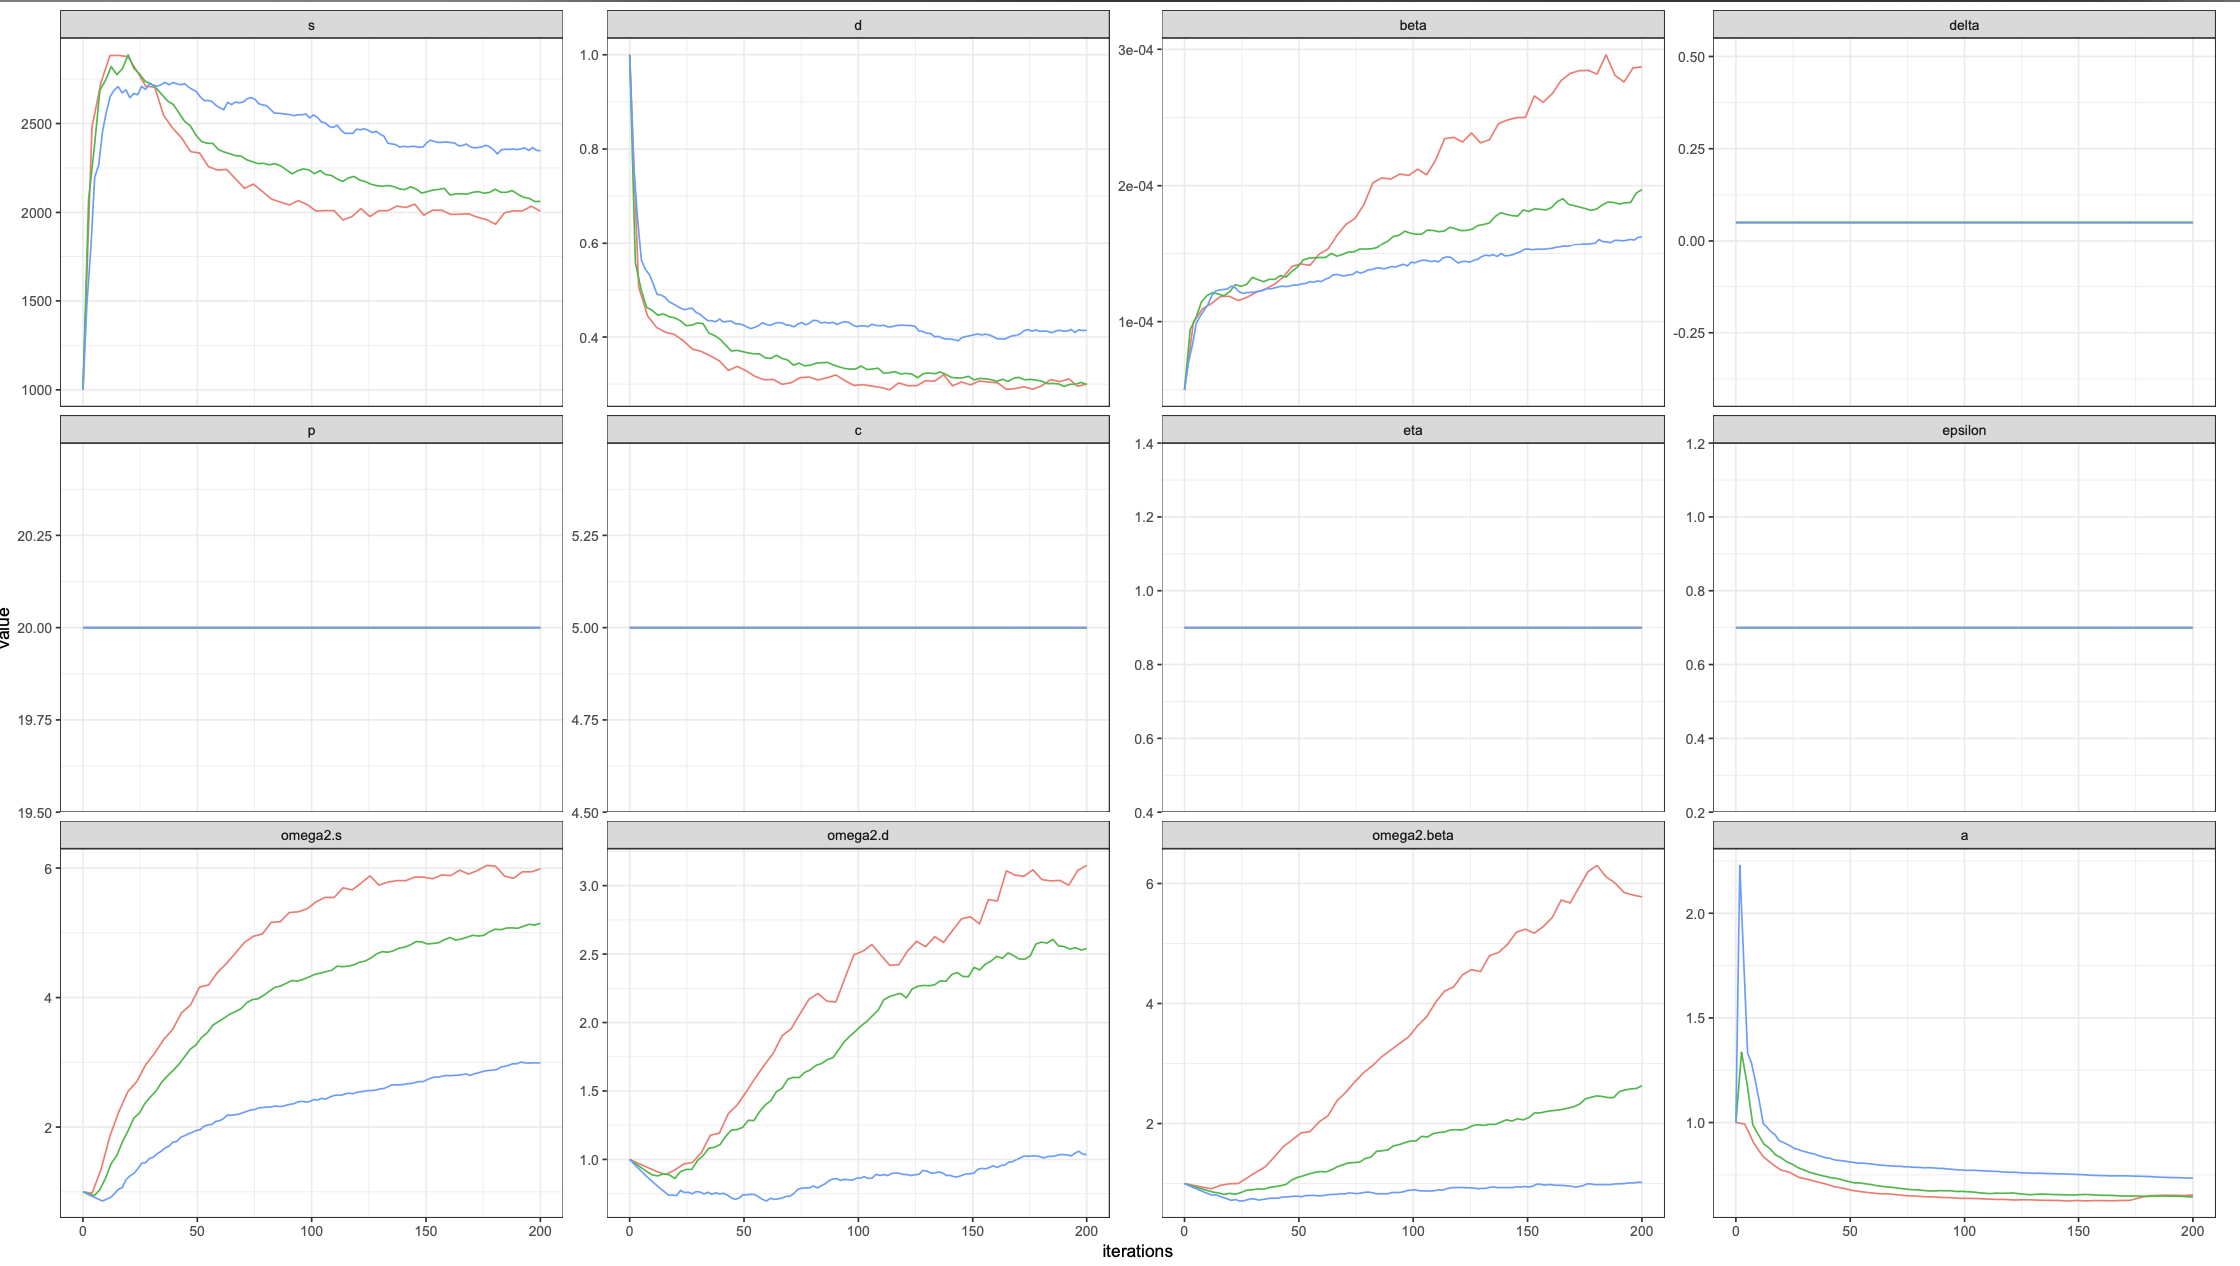
\includegraphics[width=\textwidth]{fig/hiv-dist}
\caption{Nonlinear model for HIV data.}
\label{fig:hiv}
\end{figure}


\begin{figure}[h]
\centering
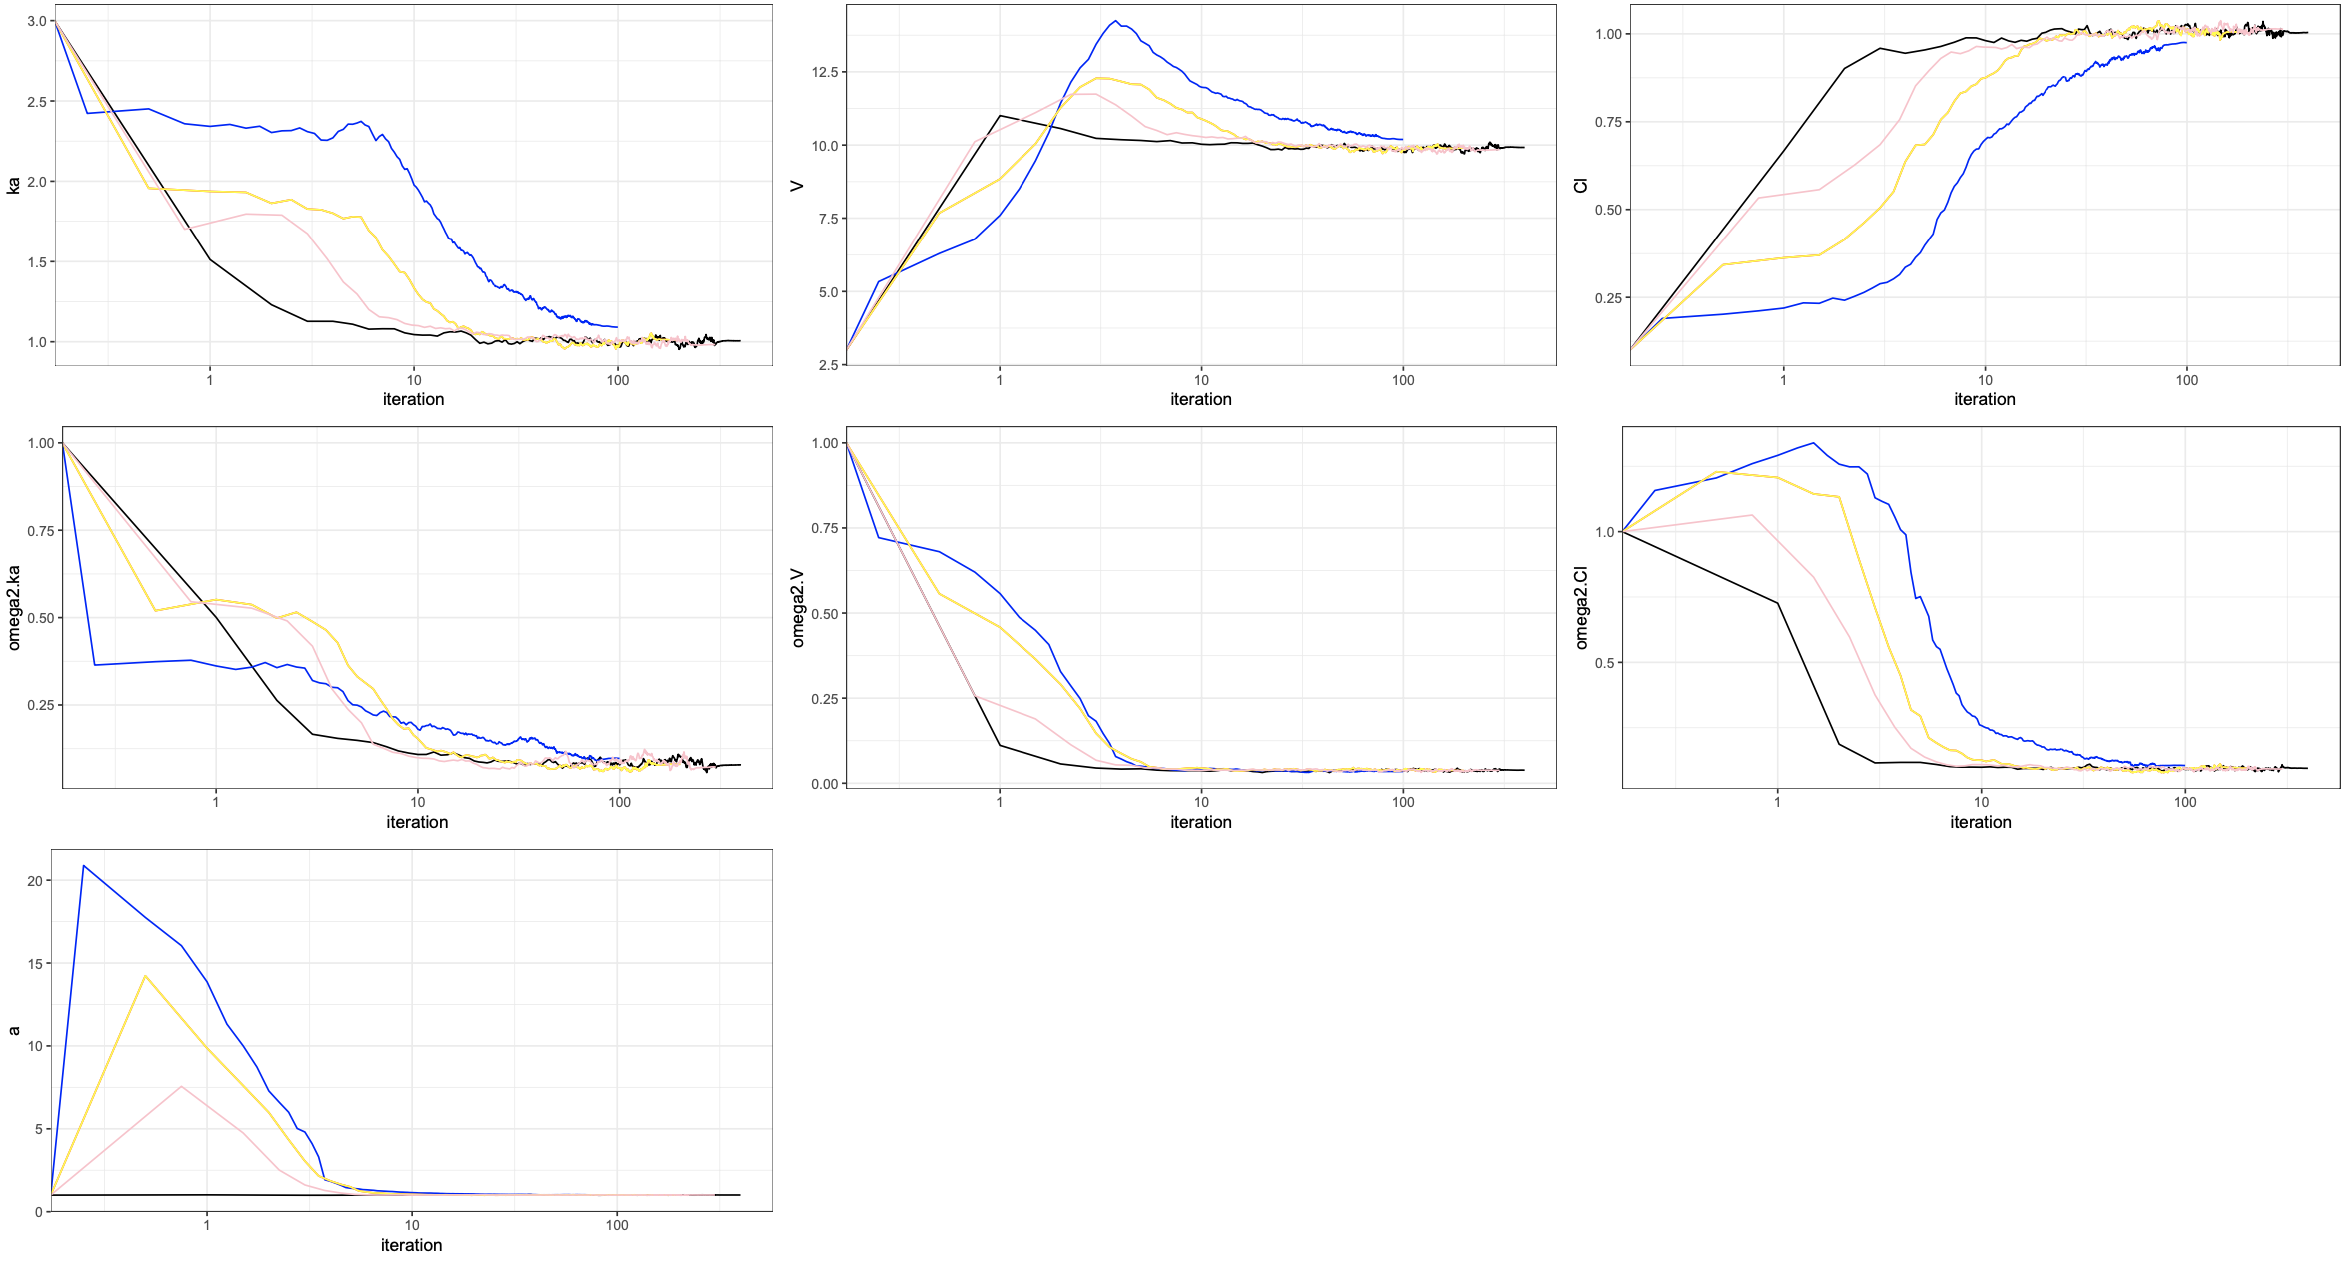
\includegraphics[width=\textwidth]{fig/pk-dist}
\caption{Nonlinear model for Warfarin data.}
\label{fig:PK}
\end{figure}

While the distributed method converges in both cases, it is quite slow in terms of iterations. I don't know if it's normal but I am investigating it right now.

\section{STANLey paper}

For the STANLey project, I have made improvements on the overleaf paper and point you to the paper itself to see the substantial progress.
In short, I have made sure we present three types of experiments: 1) toy case (Mixture model retrieval), 2) Image generation (FID and visual for CIFAR and Flowers) and 3) Image inpaintings (FID for Celeb done, need to do visual check for the baselines (running now)).
AAAI template has been used on overleaf for the next month deadline.

\textcolor{purple}{Please refer to the paper on overleaf as most of the improvements are there}.

\bibliographystyle{plain}
\bibliography{ref}


\end{document} 